\documentclass[a4paper,11pt]{article}
%
% HOW TO USE THIS TEMPLATE:
%
% MODIFY THE VALUE BELOW TO MAKE IT REFLECT THE CURRENT PROBLEM SET NUMBER
% (FOR EXAMPLE, FOR PROBLEM SET XX, THE LINE BELOW SHOULD BE: \def\mynumber{XX})
  \def\mynumber{5}
% 
% MODIFY THE VALUE BELOW TO MAKE IT REFLECT THE NUMBER OF PROBLEMS IN THE CURRENT PROBLEM SET
% (FOR EXAMPLE, IF THE CURRENT PROBLEM SET CONTAINS YY PROBLEMS, THE LINE BELOW SHOULD BE: \def\myproblemsnbr{YY})
  \def\myproblemsnbr{3}
%
%
%
%
%   ENTER THE LAST NAMES (AND ONLY LAST NAMES) OF ALL THE TEAM MEMBERS BELOWS
  \def\myname{K\"ung, Pirelli, Schubert, Dousse, Vu}
% REPLACE Doe, Smith, and Wilson WITH YOUR LAST NAMES
% NOTE: IF YOUR LAST NAME HAS ACCENTS, SOME LaTeX COMMANDS ARE:
%       for diaeresis/umlaut ", as in German, use \"a, \"u, \"o, etc.
%       for grave accent `, use \`e, \`a, \`u
%       for acute accent ', use \'a, \'e, \'u
%       for tilde ~, use \tilde{a}, \tilde{o}
%       for caret ^, use \hat{e}, \hat{o}
%	    if you need an accent on an i, say an umlaut, use \"\i{}
%		the \i{} is an i without its dot; e.g., na\"\i{}ve
%	    these all work well with lower-case letters,
%	        but only so-so with upper-case letters
%

% FOR EACH PROBLEM IN THE SET, WRITE YOUR SOLUTION IN A FILE
%   NAMED "problem1.tex", "problem2.tex", etc.
%   THESE SOLUTIONS FILES HAVE NO PREAMBLE AND
%   NO \begin{document} \end{document}
%   (THEY JUST GET INLINED WHEN RUNNING LaTeX)
%
% PLACE THESE SOLUTIONS FILES AND THE TEMPLATE IN THE SAME DIRECTORY
%
% RUN LaTeX
%
% IF ADDITIONAL PACKAGES ARE NEEDED, UNCOMMENT LINE BELOW
% AND ENTER THE PACKAGE NAMES
\usepackage{tikz}
\usepackage{booktabs}
\usepackage{float}
\usepackage{ amssymb }
\usepackage{amsmath}
\usepackage{array}
\usetikzlibrary{automata, arrows}


% DO NOT MODIFY ANYTHING BELOW THIS LINE
%%%%%

 \newcounter{problems}

  \setcounter{problems}{\myproblemsnbr}

  \usepackage{times,amsmath,amssymb,pslatex,graphicx,ifthen}
  \newcounter{problem}
  \setcounter{problem}{0}
  \makeatletter
  \def\ps@headings{%
    \let\@mkboth\markboth
    \def\@evenfoot{\hfil\large\sf Set \mynumber, Problem \theproblem\hfil}
    \def\@oddfoot{\@evenfoot}
    \def\@evenhead{\large\sc\myname\hfil\it\today\hfil\sf P.~\thepage}
    \def\@oddhead{\@evenhead}}
  \makeatother
  \pagestyle{headings}
  \advance\textwidth by16mm
  \advance\oddsidemargin by-8mm
  \advance\textheight by10mm
%%%%%

\begin{document}

\ifthenelse{\equal{\theproblems}{2}}{%
\begin{center}
  \LARGE\sf
  \begin{tabular}{||c|c||}
    \hline\hline
    Prob.~1 & Prob.~2 \\
    \hline
    &\\
    \hline\hline
  \end{tabular}
\end{center}}{}
\ifthenelse{\equal{\theproblems}{3}}{%
\begin{center}
  \LARGE\sf
  \begin{tabular}{||c|c|c||}
    \hline\hline
    Prob.~1 & Prob.~2 & Prob.~3 \\
    \hline
    &&\\
    \hline\hline
  \end{tabular}
\end{center}}{}
\ifthenelse{\equal{\theproblems}{4}}{%
\begin{center}
  \LARGE\sf
  \begin{tabular}{||c|c|c|c||}
    \hline\hline
    Prob.~1 & Prob.~2 & Prob.~3 & Prob.~4\\
    \hline
    &&&\\
    \hline\hline
  \end{tabular}
\end{center}}{}
\ifthenelse{\equal{\theproblems}{5}}{%
\begin{center}
  \LARGE\sf
  \begin{tabular}{||c|c|c|c|c||}
    \hline\hline
    Prob.~1 & Prob.~2 & Prob.~3 & Prob.~4 & Prob.~5\\
    \hline
    &&&&\\
    \hline\hline
  \end{tabular}
\end{center}}{}
\ifthenelse{\equal{\theproblems}{6}}{%
\begin{center}
  \LARGE\sf
  \begin{tabular}{||c|c|c|c|c|c||}
    \hline\hline
    Prob.~1 & Prob.~2 & Prob.~3 & Prob.~4 & Prob.~5 & Prob.~6\\
    \hline
    &&&&&\\
    \hline\hline
  \end{tabular}
\end{center}}{}
\ifthenelse{\equal{\theproblems}{7}}{%
\begin{center}
  \LARGE\sf
  \begin{tabular}{||c|c|c|c|c|c|c||}
    \hline\hline
    Prob.~1 & Prob.~2 & Prob.~3 & Prob.~4 & Prob.~5 & Prob.~6 & Prob.~7\\
    \hline
    &&&&&&\\
    \hline\hline
  \end{tabular}
\end{center}}{}
\ifthenelse{\equal{\theproblems}{8}}{%
\begin{center}
  \LARGE\sf
  \begin{tabular}{||c|c|c|c|c|c|c|c||}
    \hline\hline
    Prob.~1 & Prob.~2 & Prob.~3 & Prob.~4 & Prob.~5 & Prob.~6 & Prob.~7 & Prob.~8\\
    \hline
    &&&&&&&\\
    \hline\hline
  \end{tabular}
\end{center}}{}

\bigskip

\begin{flushleft}
{\Large Team members: \myname}
\end{flushleft}


\bigskip


%%%%%%%%%%%%%%%%%%%%%%%%%%%%%%%%%%%%%%%%%%%%%%%%%%%%%%%%%%%%
\begin{flushleft}
  \addtocounter{problem}{1}
  \large\sf Problem \theproblem .
\end{flushleft}

% YOUR SOLUTION TO PROBLEM 1 GOES HERE
% THE LATEX CODE YOU PUT HERE WILL BE INLINED (IF YOU NEED ADD ANY PACKAGES DO IT IN THE MAIN TEMPLATE FILE)

Let us prove that \textit{TWICE\_SAT} is NP-complete by reducing 3SAT to it.
Given a 3CNF formula $\phi$ with $k$ variables, we create the formula $\phi' := \phi\ and\ (x_{(k+1)}\ or \ not\ (x_{(k+1)})$.
Clearly, if $\phi$ has at least one satisfying assignment, $\phi'$ must have at least two satisfying assignment, one where $x_{(k+1)}$ is true and one where it is false.
Therefore, \textit{TWICE\_SAT} can be reduced to 3SAT, which means \textit{TWICE\_SAT} is NP-complete.
\addtocounter{problems}{-1}

%%%%%%%%%%%%%%%%%%%%%%%%%%%%%%%%%%%%%%%%%%%%%%%%%%%%%%%%%%%%
\newpage
\begin{flushleft}
  \addtocounter{problem}{1}
  \large\sf Problem \theproblem .
\end{flushleft}

% YOUR SOLUTION TO PROBLEM 2 GOES HERE
% THE LATEX CODE YOU PUT HERE WILL BE INLINED (IF YOU NEED ADD ANY PACKAGES DO IT IN THE MAIN TEMPLATE FILE)


Since $L$ is regular, there is a DFA $M$ that can match $L$. Let us create an NFA $M'$ that can match $L^R$, which will prove that $L^R$ is regular.
$M'$ is composed of all of $M$'s states, plus one new state. This new state is the start state of the NFA, and it contains only $\epsilon$ transitions to all states that were accepting states of $M$. The accepting state of $M'$ is the start state of $M$. The transition function of $M'$ is the opposite of $M$; if an input $x$ caused $M$ to go from $q_0$ to $q_1$, it causes $M'$ to go from $q_1$ to $q_0$.

To express it more formally:
\begin{align*}
M &= (Q, \Sigma, \delta, s, F) \\
M' &= (Q', \Sigma, \delta;, s', F') \\
s' &= \text{new state, connected to the end of all the states }F \\
Q' &= Q + \{ s' \} \\
F' &= \{ s \} \\
\delta' &= \delta^R \\
\delta'(q,x) &= \left\{ 
  \begin{array}{l l}
    F & \quad \text{if } q = s' \\
    \{q_2 | \delta(q_2,x)\} = q & \quad \text{otherwise}
  \end{array} \right.
\end{align*}

%\begin{figure}[H]
%\centering
%\begin{tikzpicture}[shorten >=2pt, auto, node distance=2 cm, scale = 1, transform shape]
%    
%\node[state, initial] (q0) {$q_0$};
%\node[state] (anon0) [right of=q0, xshift=0.3cm, yshift=0.4cm] {};
%\node[state] (anon1) [right of=q0, xshift=1.3cm, yshift=-0.8cm] {};
%\node[state] (anon2) [right of=q0, xshift=1.7cm, yshift=1.5cm] {};
%\node[state, accepting] (anon3) [right of=q0, xshift=3.3cm, yshift=1.8cm] {};
%\node[state, accepting] (anon4) [right of=q0, xshift=2.9cm, yshift=-0.8cm] {};
%\node[draw=none,fill=none] (inv1)[right of=q0, yshift=1.3cm]{};
%\node[draw=none,fill=none] (inv2) [right of=q0, yshift=-1.3cm]{};
%\node [draw=black, fit = (anon0)(anon1)(anon2)(anon3)(anon4), inner sep=0.50cm]{};
%
%\path[->] (q0) edge node [align=center] {} (inv1);
%\path[->] (q0) edge node [align=center] {} (inv2);
%
%\end{tikzpicture}
%\caption{DFA $A_1$}
%\end{figure}
%
%
%\begin{figure}[H]
%\centering
%\begin{tikzpicture}[shorten >=2pt, auto, node distance=2 cm, scale = 1, transform shape]
%    
%\node[state, accepting] (q0) {};
%\node[state] (anon0) [right of=q0, xshift=0.3cm, yshift=0.4cm] {};
%\node[state] (anon1) [right of=q0, xshift=1.3cm, yshift=-0.8cm] {};
%\node[state] (anon2) [right of=q0, xshift=1.7cm, yshift=1.5cm] {};
%\node[state] (anon3) [right of=q0, xshift=3.3cm, yshift=1.8cm] {};
%\node[state] (anon4) [right of=q0, xshift=2.9cm, yshift=-0.8cm] {};
%\node[state, initial] (s0) [right of=q0, xshift=8cm]{$q'_0$};
%
%\node[draw=none,fill=none] (inv1)[right of=q0, yshift=1.3cm]{};
%\node[draw=none,fill=none] (inv2) [right of=q0, yshift=-1.3cm]{};
%\node [draw=black, fit = (anon0)(anon1)(anon2)(anon3)(anon4), inner sep=0.50cm]{};
%
%\path[<-] (q0) edge node [align=center] {} (inv1);
%\path[<-] (q0) edge node [align=center] {} (inv2);
%\path[<-] (q0) edge node [align=center] {} (inv1);
%\path[<-] (q0) edge node [align=center] {} (inv2);
%
%\end{tikzpicture}
%\caption{DFA $A_1$}
%\end{figure}


\begin{figure}[H]
\centering
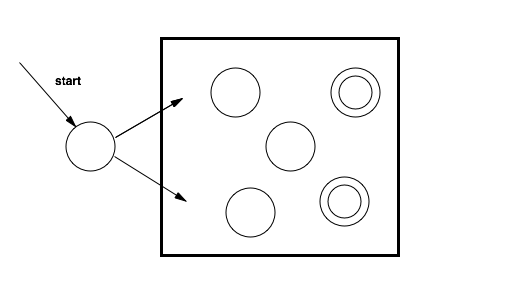
\includegraphics[scale=0.6]{original_dfa}
\caption{Original DFA $M$}
\end{figure}


\begin{figure}[H]
\centering
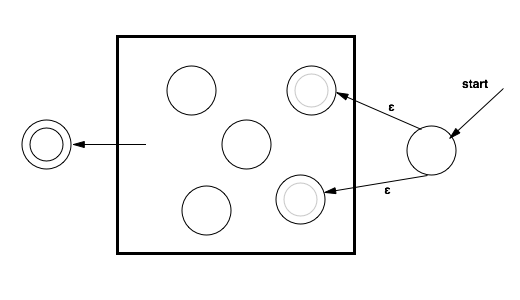
\includegraphics[scale=0.6]{NFA}
\caption{New NFA $M'$}
\end{figure}


This new machine $M'$ will be able to read every word the original machine $M$ was able to read, in the opposite direction; indeed, for every word $M$ was able to read it ended up in one of the accepting states to which $M'$ can transition to at no cost ($\epsilon$) from the start and therefore will end up after the reverse read of the word in the initial state of $M$, meaning in the accepting state of $M'$.



\addtocounter{problems}{-1}

%%%%%%%%%%%%%%%%%%%%%%%%%%%%%%%%%%%%%%%%%%%%%%%%%%%%%%%%%%%%
\ifthenelse{\equal{\theproblems}{0}}
{}%
{%
\newpage
\begin{flushleft}
  \addtocounter{problem}{1}
  \large\sf Problem \theproblem .
\end{flushleft}

% YOUR SOLUTION TO PROBLEM 3 (IF THERE IS ONE) GOES HERE
% THE LATEX CODE YOU PUT HERE WILL BE INLINED (IF YOU NEED ADD ANY PACKAGES DO IT IN THE MAIN TEMPLATE FILE)

We want to prove the following:

\begin{align*}
\frac {L}{2} :=& \{x \in \Sigma * | \exists y : yx \in L, |x| = |y| \}
\end{align*}

We haven proven in problem 2 that the inverse of a regular language is regular. Let's assume we have some way of proving that the first half of a language is regular; we could prove that the first half of a reversed language is regular, which would also mean that the reverse of the first half of a reversed language is regular. A bit tricky, but it does correspond to the second half.

Let us prove our assumption; that the first half of a regular language is regular.


Let $L$ be a regular language. Let $half(L) := \{ x | \exists y : xy \in L, |x| = |y| \}$. We want to prove that $half(L)$ is regular.

Let $M < Q, \Sigma, \delta, q_0, F>$ be a DFA that accepts $L$, which must exist because $L$ is regular. Supposing that $\hat \delta (q_0, x) = q_i$, i.e. the input $x$ leads $M$ to the state $q_i$, we must check if $\exists y : |y| = |x|$ that satisfies $\hat \delta (q_i, y) \in F$. 

Let $S_n \subset Q$ be the set of states that lead to an accepting state for some input (not necessarily any input) of length n. 
It is clear that for $x$ of length $n$ and $\hat \delta(q_0, x) = q_i$, $q_i \in S_n \rightarrow x \in \frac L 2$.  $(*)$ \newline

$S_0 = F$, since by definition of $S_n$ there are no more steps needed. $S_{n+1}$ can be easily computed from $S_n$ and $\delta$; it is the set of states that can transition to a state in $S_n$.
We need a DFA that will keep track of $S_n$ as we go through $L$. Let $M'$ be a new DFA whose states are in $(Q, Q*)$ i.e. they're pairs of one state in $Q$ and a set of states in $Q$. The transition function $\delta'$ of $M'$ takes an input $x$ of length $n$ and yields $(\hat \delta(q_0, x), S_n)$. \newline

The start state of $M'$ is $(q_0, F)$, and the accepting states are $(q, S) \in (Q, Q^*)$ where $q \in S$; in common English, "the states reached after n inputs that can also reach an accepting state after n inputs". \newline
$(*)$ above allows us to show that $M'$ indeed accepts $half(L)$, and therefore $half(L)$ is regular.

(source/inspiration for the $half(L)$ proof: \url{http://www-bcf.usc.edu/~breichar/teaching/2011cs360/half\%28L\%29example.pdf})

\addtocounter{problems}{-1}
}
%%%%%%%%%%%%%%%%%%%%%%%%%%%%%%%%%%%%%%%%%%%%%%%%%%%%%%%%%%%%
\ifthenelse{\equal{\theproblems}{0}}
{}%
{%
\newpage
\begin{flushleft}
  \addtocounter{problem}{1}
  \large\sf Problem \theproblem .
\end{flushleft}

\input{problem4.tex}
\addtocounter{problems}{-1}
}
%%%%%%%%%%%%%%%%%%%%%%%%%%%%%%%%%%%%%%%%%%%%%%%%%%%%%%%%%%%%%%%%%%
\ifthenelse{\equal{\theproblems}{0}}
{}%
{%
\newpage
\begin{flushleft}
  \addtocounter{problem}{1}
  \large\sf Problem \theproblem .
\end{flushleft}

\input{problem5.tex}
\addtocounter{problems}{-1}
}
%%%%%%%%%%%%%%%%%%%%%%%%%%%%%%%%%%%%%%%%%%%%%%%%%%%%%%%%%%%%
\ifthenelse{\equal{\theproblems}{0}}
{}%
{%
\newpage
\begin{flushleft}
  \addtocounter{problem}{1}
  \large\sf Problem \theproblem .
\end{flushleft}

\input{problem6.tex}
\addtocounter{problems}{-1}
}
%%%%%%%%%%%%%%%%%%%%%%%%%%%%%%%%%%%%%%%%%%%%%%%%%%%%%%%%%%%%
\ifthenelse{\equal{\theproblems}{0}}
{}%
{%
\newpage
\begin{flushleft}
  \addtocounter{problem}{1}
  \large\sf Problem \theproblem .
\end{flushleft}

\input{problem7.tex}
\addtocounter{problems}{-1}
}
%%%%%%%%%%%%%%%%%%%%%%%%%%%%%%%%%%%%%%%%%%%%%%%%%%%%%%%%%%%%
\ifthenelse{\equal{\theproblems}{0}}
{}%
{%
\newpage
\begin{flushleft}
  \addtocounter{problem}{1}
  \large\sf Problem \theproblem .
\end{flushleft}

\input{problem8.tex}
\addtocounter{problems}{-1}
}
\end{document}
